%%%%%%%%%%%%%%%%%%%%%%%%%%%%%%%%%%%%%%%%%%%%%%%%%%%%%%%%%%%%%%%
%
% Welcome to Overleaf --- just edit your LaTeX on the left,
% and we'll compile it for you on the right. If you open the
% 'Share' menu, you can invite other users to edit at the same
% time. See www.overleaf.com/learn for more info. Enjoy!
%
%%%%%%%%%%%%%%%%%%%%%%%%%%%%%%%%%%%%%%%%%%%%%%%%%%%%%%%%%%%%%%%
\documentclass[11pt]{article}

%%%%%%%%%%%%%%%%%%%%%%%%%%%%%%%%%%%%%%%%%%%%%%%%%%%%%%%%%%%%%%%
%                      Customize Header                       %
%%%%%%%%%%%%%%%%%%%%%%%%%%%%%%%%%%%%%%%%%%%%%%%%%%%%%%%%%%%%%%%

\newcommand{\assessmentTitle}{
CheckIt Assessment
}
\newcommand{\assessmentVersion}{
Version 1770002163466
}
\newcommand{\assessmentInstructions}{
Do not use any unapproved aids while taking this assessment.
Read each question carefully and be sure to show all work
in the space provided.
}

%%%%%%%%%%%%%%%%%%%%%%%%%%%%%%%%%%%%%%%%%%%%%%%%%%%%%%%%%%%%%%%
%%%%%%%%%%%%%%%%%%%%%%%%%%%%%%%%%%%%%%%%%%%%%%%%%%%%%%%%%%%%%%%



\usepackage{amsfonts,amssymb,amsmath,amsthm}
\setcounter{MaxMatrixCols}{50}
\usepackage{hyperref}
\let\oldhref\href\renewcommand{\href}[2]{\oldhref{#1}{#2}\footnote{\url{#1}}}
\usepackage[margin=1in,tmargin=2in,headheight=84pt]{geometry}
\usepackage{enumerate}
\usepackage{graphicx}
\usepackage{fancyhdr}
\usepackage{lastpage}
\pagestyle{fancy}
\fancyhf{}
\rhead{Name: \underline{\hspace{2.5in}}\\ID: \underline{\hspace{2.5in}}

\vspace{2.5em}}
\chead{\vspace{2.5em}

\fbox{\fbox{\parbox{6in}{\centering\assessmentInstructions}}}}
\lhead{\assessmentTitle \hspace{2em} \assessmentVersion

\vspace{2.5em}}
\rfoot{Page \thepage\ of \pageref{LastPage}}
\setlength{\headheight}{80pt}
\renewcommand{\headrulewidth}{0pt}


\begin{document}

\begin{enumerate}

% 

\item %%%%% SpaTeXt Commands %%%%%
\providecommand{\stxKnowl}{}\renewcommand{\stxKnowl}[1]{#1}
\providecommand{\stxOuttro}{}\renewcommand{\stxOuttro}[1]{#1}
\providecommand{\stxTitle}{}\renewcommand{\stxTitle}[1]{#1}
% Comment next line to show outtros
\renewcommand{\stxOuttro}[1]{}
%%%%%%%%%%%%%%%%%%%%%%%%%%%%
\stxKnowl{
Evaluate the function \(f(x) = -x^{2} + 6 \, x - 1\).

\begin{enumerate}
\item
\stxKnowl{
Find \(f(-5)\).

\stxOuttro{
SOLUTION

\(-1(-5)^2 + 6(-5) + -1\)

\(\boxed{f(-5) = -56}\)

}
}

\item
\stxKnowl{
Find \(f(-x)\).

\stxOuttro{
SOLUTION

\(-1(-x)^2 + 6(-x) + -1\)

\(\boxed{f(-x) = -x^{2} - 6 \, x - 1}\)

}
}

\item
\stxKnowl{
Find \(f(x + a)\).

\stxOuttro{
SOLUTION

\(-1(x+a)^2 + 6(x+a) + -1\)

\(\boxed{f(x + a) = -a^{2} - 2 \, a x - x^{2} + 6 \, a + 6 \, x - 1}\)

}
}

\end{enumerate}
}

\newpage

% 

\item %%%%% SpaTeXt Commands %%%%%
\providecommand{\stxKnowl}{}\renewcommand{\stxKnowl}[1]{#1}
\providecommand{\stxOuttro}{}\renewcommand{\stxOuttro}[1]{#1}
\providecommand{\stxTitle}{}\renewcommand{\stxTitle}[1]{#1}
% Comment next line to show outtros
\renewcommand{\stxOuttro}[1]{}
%%%%%%%%%%%%%%%%%%%%%%%%%%%%
\stxKnowl{
 Determine the number and type of solutions for the following equation: 

 \(x^{2} + 9 \, x - 3 = -2 \, x\) 

\stxOuttro{
SOLUTION

 \(1x^2 + (11)x + -3 = 0\) 

 \(\Delta = (11)^2 - 4(1)(-3)\) 

 \(\Delta = 133\) 

 \(\boxed{\text{ two solutions, unequal real roots }}\) 

}
}

\newpage

% 

\item %%%%% SpaTeXt Commands %%%%%
\providecommand{\stxKnowl}{}\renewcommand{\stxKnowl}[1]{#1}
\providecommand{\stxOuttro}{}\renewcommand{\stxOuttro}[1]{#1}
\providecommand{\stxTitle}{}\renewcommand{\stxTitle}[1]{#1}
% Comment next line to show outtros
\renewcommand{\stxOuttro}[1]{}
%%%%%%%%%%%%%%%%%%%%%%%%%%%%
\stxKnowl{
Solve for all solutions. Identify any extraneous solutions.

 \(x^{2} - 4 \, x + 7 = 0\) 

\stxOuttro{
SOLUTION

 \(x = \frac{-(-4) \pm \sqrt{(-4)^2 - 4(1)(7)}}{2(1)}\) 

 \(= \frac{4 \pm \sqrt{16 - 28}}{2}\) 

 \(= \frac{4 \pm \sqrt{-12}}{2}\) 

 \(= \frac{4 \pm 2i\sqrt{3}}{2}\) 

 \(= \frac{2(2 \pm i\sqrt{3})}{2}\) 

 \(\boxed{x = 2 \pm i\sqrt{3}}\) 

 (No extraneous solutions) 

}
}

\newpage

% 

\item %%%%% SpaTeXt Commands %%%%%
\providecommand{\stxKnowl}{}\renewcommand{\stxKnowl}[1]{#1}
\providecommand{\stxOuttro}{}\renewcommand{\stxOuttro}[1]{#1}
\providecommand{\stxTitle}{}\renewcommand{\stxTitle}[1]{#1}
% Comment next line to show outtros
\renewcommand{\stxOuttro}[1]{}
%%%%%%%%%%%%%%%%%%%%%%%%%%%%
\stxKnowl{
Solve for all solutions. Identify any extraneous solutions.

 \(\sqrt{x + 9} - 9 = -7\) 

\stxOuttro{
SOLUTION

 \(\sqrt{x + 9} = 2\) 

 \(x + 9 = 4\) 

 \(x = 4 - 9\) 

 \(\boxed{x = -5}\) 

 (No extraneous solutions) 

}
}

\newpage

% 

\item %%%%% SpaTeXt Commands %%%%%
\providecommand{\stxKnowl}{}\renewcommand{\stxKnowl}[1]{#1}
\providecommand{\stxOuttro}{}\renewcommand{\stxOuttro}[1]{#1}
\providecommand{\stxTitle}{}\renewcommand{\stxTitle}[1]{#1}
% Comment next line to show outtros
\renewcommand{\stxOuttro}[1]{}
%%%%%%%%%%%%%%%%%%%%%%%%%%%%
\stxKnowl{
 Solve the rational equation for all solutions. Identify any extraneous solutions. 

 \(\displaystyle \frac{x}{x + 2} - \frac{12}{(x + 2)(x - 4)} = \frac{-15}{x - 4}\) 

\stxOuttro{
SOLUTION

 \(x(x - 4) - 12 = -15(x + 2)\) 

 \(x^{2} + 11 \, x + 18 = 0\) 

 \((x + 2)(x + 9) = 0\) 

 \(x = -9, \quad x = -2\) 

 \(x = -2 \implies \text{Extraneous}\) 

 \(\boxed{x = -9}\) 

}
}

\newpage

% 

\item %%%%% SpaTeXt Commands %%%%%
\providecommand{\stxKnowl}{}\renewcommand{\stxKnowl}[1]{#1}
\providecommand{\stxOuttro}{}\renewcommand{\stxOuttro}[1]{#1}
\providecommand{\stxTitle}{}\renewcommand{\stxTitle}[1]{#1}
% Comment next line to show outtros
\renewcommand{\stxOuttro}[1]{}
%%%%%%%%%%%%%%%%%%%%%%%%%%%%
\stxKnowl{
 Given that the function is one-to-one, find the inverse function \(f^{-1}(x)\). 

 \(f(x) = \sqrt[3]{x + 1} - 1\) 

\stxOuttro{
SOLUTION

 \(y = f(x) = \sqrt[3]{x + 1} - 1\) 

 \(x = \sqrt[3]{y + 1} - 1\) 

 \(x + 1 = \sqrt[3]{y + 1}\) 

 \((x + 1)^3 = y + 1\) 

 \(y = (x + 1)^3 - 1\) 

 \(\boxed{ f^{-1}(x) = (x + 1)^3 - 1 }\) 

  

 \(= (x + 1)(x^2 + 2x + 1) - 1\) 

 \(\boxed{ f^{-1}(x) = x^{3} + 3 \, x^{2} + 3 \, x }\) 

}
}

\newpage

% 

\item %%%%% SpaTeXt Commands %%%%%
\providecommand{\stxKnowl}{}\renewcommand{\stxKnowl}[1]{#1}
\providecommand{\stxOuttro}{}\renewcommand{\stxOuttro}[1]{#1}
\providecommand{\stxTitle}{}\renewcommand{\stxTitle}[1]{#1}
% Comment next line to show outtros
\renewcommand{\stxOuttro}[1]{}
%%%%%%%%%%%%%%%%%%%%%%%%%%%%
\stxKnowl{
Suppose a rocket carrying fireworks is launched from a hill 69 feet above a lake. The rocket's height \(h\) (in feet) above the lake at time \(t\) (in seconds) is given by

 \(h(t) = -16t^2 + 96t + 69\) 

\begin{enumerate}
\item
\stxKnowl{
When will the rocket reach its maximum height?

\stxOuttro{
SOLUTION

 \(t = \frac{-96}{2(-16)} = \frac{-96}{-32}\) 

 \(\boxed{t = 3 \text{ sec}}\) 

}
}

\item
\stxKnowl{
What is the maximum height the rocket will reach?

\stxOuttro{
SOLUTION

 \(h(3) = -16(3)^2 + 96(3) + 69\) 

 \(= -144 + 288 + 69\) 

 \(\boxed{h = 213 \text{ ft}}\) 

}
}

\item
\stxKnowl{
Interpret your results for the previous two questions in one or more complete sentences, including appropriate units.

\stxOuttro{
SOLUTION

The rocket will reach a maximum height of 213 ft 3 seconds after launch.

}
}

\end{enumerate}
}

\newpage

% 

\item %%%%% SpaTeXt Commands %%%%%
\providecommand{\stxKnowl}{}\renewcommand{\stxKnowl}[1]{#1}
\providecommand{\stxOuttro}{}\renewcommand{\stxOuttro}[1]{#1}
\providecommand{\stxTitle}{}\renewcommand{\stxTitle}[1]{#1}
% Comment next line to show outtros
\renewcommand{\stxOuttro}[1]{}
%%%%%%%%%%%%%%%%%%%%%%%%%%%%
\stxKnowl{
 Given \(f(x) = 2 \, x\) and \(g(x) = -2 \, x^{2} + 3\), find the following: 

\begin{enumerate}
\item
\stxKnowl{
\((f \circ g)(x)\)

\stxOuttro{
SOLUTION

 \(f(g(x)) = 2(-2 \, x^{2} + 3)\) 

 \(\boxed{ -4 \, x^{2} + 6 }\) 

ERROR 1: \(g(f(x))\)

 \(= -2(2 \, x)^2 + 3\) 

 \(= -2(4 \, x^{2}) + 3\) 

 \(\boxed{ -8 \, x^{2} + 3 }\) 

ERROR 2: \(f(x) \cdot g(x)\)

 \(= (2 \, x)(-2 \, x^{2} + 3)\) 

 \(\boxed{ -4 \, x^{3} + 6 \, x }\) 

}
}

\item
\stxKnowl{
\((f \circ f)(x)\)

\stxOuttro{
SOLUTION

 \(f(f(x)) = 2(2 \, x)\) 

 \(\boxed{ 4 \, x }\) 

}
}

\end{enumerate}
}

\newpage

% 

\item %%%%% SpaTeXt Commands %%%%%
\providecommand{\stxKnowl}{}\renewcommand{\stxKnowl}[1]{#1}
\providecommand{\stxOuttro}{}\renewcommand{\stxOuttro}[1]{#1}
\providecommand{\stxTitle}{}\renewcommand{\stxTitle}[1]{#1}
% Comment next line to show outtros
\renewcommand{\stxOuttro}[1]{}
%%%%%%%%%%%%%%%%%%%%%%%%%%%%
\stxKnowl{
 Evaluate the difference quotient, \(\displaystyle{ \frac{f(x+h)-f(x)}{h}}\) , for \(f(x) = x^{2} - 3\). 

\stxOuttro{
SOLUTION

 \(f(x+h) = 1(x+h)^2 - 3\) 

 \(= 1(x^2 + 2xh + h^2) - 3\) 

 \(= h^{2} + 2 \, h x + x^{2} - 3\) 

 \(\displaystyle{\frac{f(x+h)-f(x)}{h} = \frac{ (h^{2} + 2 \, h x + x^{2} - 3) - (x^{2} - 3) }{h}}\) 

 \(=\displaystyle{ \frac{ h^{2} + 2 \, h x }{h}}\) 

 \(= \displaystyle{ \frac{ h(h + 2 \, x) }{h}}\) 

 \(\boxed{ h + 2 \, x }\) 

}
}

\newpage

% 

\item %%%%% SpaTeXt Commands %%%%%
\providecommand{\stxKnowl}{}\renewcommand{\stxKnowl}[1]{#1}
\providecommand{\stxOuttro}{}\renewcommand{\stxOuttro}[1]{#1}
\providecommand{\stxTitle}{}\renewcommand{\stxTitle}[1]{#1}
% Comment next line to show outtros
\renewcommand{\stxOuttro}[1]{}
%%%%%%%%%%%%%%%%%%%%%%%%%%%%
\stxKnowl{
 Consider the function: 

 \(f(x) = \frac{1}{4}(x - 4)^2 -9\) 

 Find the following properties: 

\begin{itemize}
\item
Vertex

\item
Axis of Symmetry

\item
\(x\)-intercepts

\item
\(y\)-intercept

\item
Domain

\item
Range

\end{itemize}
\stxOuttro{
SOLUTION

 \(\textbf{Direction: } \text{Opens Up}\) 

 \(\textbf{Vertex: } (4, -9)\) 

 \(\textbf{Axis of Symmetry: } x = 4\) 

 \(\textbf{x-intercepts:}\) 

 \(\frac{1}{4}(x - 4)^2 -9 = 0\) 

 \((x - 4)^2 = 36\) 

 \(x = 4 \pm 6\) 

 \(\boxed{ -2, 10 }\) 

 \(\textbf{y-intercept:}\) 

 \(= \frac{1}{4}(0 - 4)^2 -9\) 

 \(= \frac{1}{4}(16) -9\) 

 \(= 4 -9\) 

 \(\boxed{ -5 }\) 

 \(\textbf{Domain: } (-\infty, \infty)\) 

 \(\textbf{Range: } [-9, \infty)\) 

}
}

\newpage

% 

\item %%%%% SpaTeXt Commands %%%%%
\providecommand{\stxKnowl}{}\renewcommand{\stxKnowl}[1]{#1}
\providecommand{\stxOuttro}{}\renewcommand{\stxOuttro}[1]{#1}
\providecommand{\stxTitle}{}\renewcommand{\stxTitle}[1]{#1}
% Comment next line to show outtros
\renewcommand{\stxOuttro}[1]{}
%%%%%%%%%%%%%%%%%%%%%%%%%%%%
\stxKnowl{
 A quadratic function has the characteristics given below. Use the axis of symmetry to generate two additional points, then use all five points to graph the function. 

\begin{itemize}
\item
\(\text{Vertex: } (2, 1)\)

\item
\(x\text{-intercept: } 3\)

\item
\(y\text{-intercept: } -3\)

\end{itemize}
 \begin{tikzpicture}[scale=0.35] \draw[step=1cm, gray!40, very thin] (-10,-10) grid (10,10); \draw[thick, <->] (-10.5,0) -- (10.5,0); \draw[thick, <->] (0,-10.5) -- (0,10.5); \end{tikzpicture} 

\stxOuttro{
SOLUTION

 \begin{multicols}{2}  

\begin{itemize}
\item
\(\text{Vertex: } (2, 1)\)

\item
\(y\text{-intercept: } (0, -3)\)

\item
\(\text{Reflected } y\text{-int: } (4, -3)\)

\item
\(\text{Given Root: } (3, 0)\)

\item
\(\text{Reflected Root: } (1, 0)\)

\end{itemize}
 \columnbreak  

 \begin{tikzpicture}[scale=0.35] \draw[step=1cm, gray!40, very thin] (-10,-10) grid (10,10); \draw[thick, <->] (-10.5,0) -- (10.5,0); \draw[thick, <->] (0,-10.5) -- (0,10.5); \clip (-10,-10) rectangle (10,10); \draw[line width=1.5pt, blue!80!black, samples=100, domain=-10:10, <->] plot (\x, {-1.0*(\x - 2)^2 + 1}); \fill[blue] (2,1) circle (7pt); \fill[blue] (1,0) circle (7pt); \fill[blue] (3,0) circle (7pt); \fill[blue] (0,-3) circle (7pt); \fill[blue] (4,-3) circle (7pt); \end{tikzpicture} 

 \end{multicols} 

}
}

\newpage

% 

\item %%%%% SpaTeXt Commands %%%%%
\providecommand{\stxKnowl}{}\renewcommand{\stxKnowl}[1]{#1}
\providecommand{\stxOuttro}{}\renewcommand{\stxOuttro}[1]{#1}
\providecommand{\stxTitle}{}\renewcommand{\stxTitle}[1]{#1}
% Comment next line to show outtros
\renewcommand{\stxOuttro}[1]{}
%%%%%%%%%%%%%%%%%%%%%%%%%%%%
\stxKnowl{
 Use the table to identify the transformations described by \(g(x) = -f(x - 1) + 1\). 

 Circle the option that applies and fill in the blanks as appropriate. Then apply these transformations to the graph of the function shown below. 

 \(\renewcommand{\arraystretch}{3} \begin{array}{|l|l|} \hline \textbf{Horizontal Transformations} & \textbf{Vertical Transformations} \\ \hline \text{Reflection: YES or NO} & \text{Reflection: YES or NO} \\ \hline \text{Dilation: \underline{\hspace{2cm}} times as wide} & \text{Dilation: \underline{\hspace{2cm}} times as tall} \\ \hline \text{Translation: \underline{\hspace{2cm}} units LEFT or RIGHT} & \text{Translation: \underline{\hspace{2cm}} units UP or DOWN} \\ \hline \end{array}\) 

 \noindent\makebox[\textwidth][c]{ \begin{minipage}{0.48\textwidth} \centering \begin{tikzpicture}[scale=0.39] \draw[step=1cm, gray!40, very thin] (-10,-10) grid (10,10); \draw[thick, <->] (-10.5,0) -- (10.5,0); \draw[thick, <->] (0,-10.5) -- (0,10.5); \draw[line width=1.5pt, black] (-2,1) -- (-1,2) -- (0,0) -- (1,4) -- (3,4);\fill[black] (-2,1) circle (5pt); \fill[black] (-1,2) circle (5pt); \fill[black] (0,0) circle (5pt); \fill[black] (1,4) circle (5pt); \fill[black] (3,4) circle (5pt); \end{tikzpicture} \end{minipage} \hfill \begin{minipage}{0.48\textwidth} \centering \begin{tikzpicture}[scale=0.39] \draw[step=1cm, gray!40, very thin] (-10,-10) grid (10,10); \draw[thick, <->] (-10.5,0) -- (10.5,0); \draw[thick, <->] (0,-10.5) -- (0,10.5); \end{tikzpicture} \end{minipage} } 

\stxOuttro{
SOLUTION



\begin{itemize}
\item
 \(\textbf{Horizontal: } \text{Reflection: NO, Dilation: 1, Shift: 1 units RIGHT.}\) 

\item
 \(\textbf{Vertical: } \text{Reflection: YES, Dilation: 1, Shift: 1 units UP.}\) 

\end{itemize}


 \begin{tikzpicture}[scale=0.39] \draw[step=1cm, gray!40, very thin] (-10,-10) grid (10,10); \draw[thick, <->] (-10.5,0) -- (10.5,0); \draw[thick, <->] (0,-10.5) -- (0,10.5); \draw[line width=1.5pt, blue] (-1,0) -- (0,-1) -- (1,1) -- (2,-3) -- (4,-3);\fill[blue] (-1,0) circle (5pt); \fill[blue] (0,-1) circle (5pt); \fill[blue] (1,1) circle (5pt); \fill[blue] (2,-3) circle (5pt); \fill[blue] (4,-3) circle (5pt); \end{tikzpicture} 

}
}

\newpage

% 

\end{enumerate}

\end{document}